\documentclass[aspectratio=169]{beamer}

\usetheme{metropolis}

\usepackage[english]{babel}
\usepackage{graphicx}
\usepackage{svg}
\usepackage{float}
\usepackage{subcaption}
\usepackage{minted}

% Meta info
\title{Universal Robots UR5 Smart Outliner}
\subtitle{A ROS2 Simulation inside a Containerized environment}
\author{
    \textbf{Student:} Tommaso Cosimi \\
    \textbf{ID:} 191739
}
\date{}
\institute{
    Università degli Studi di Modena e Reggio Emilia \\
    Dipartimento di Ingegneria ``Enzo Ferrari''
}

\begin{document}
% Title Page
\maketitle

% Table of contents
\begin{frame}{Table of Contents}
    \tableofcontents
    \thispagestyle{empty}
\end{frame}

% Sections
\section{Project Overview}
\label{Sec:Project_Overview}
\begin{frame}{Project Overview}
    The Project explores the \textbf{Motion Planning} capabilities of a simulated \textbf{Universal Robots UR5} manipulator aided by \textbf{Computer Vision} techniques.

    The \textbf{Robot simulation} runs under \textbf{ROS2 Humble} accompanied by \textbf{MoveIt2} and exploiting \textbf{Gazebo 11} for a physically-accurate simulation environment, while the \textbf{Computer Vision applications} make use of both \textbf{ROS Nodes} and standalone \textbf{Python scripts}.

    All of this is running inside \textbf{Docker Containers}.
\end{frame}

\subsection{Why this Toolset}
\begin{frame}{Why ROS2?}
    \begin{columns}
        \begin{column}{.75\linewidth}
            The \textbf{discontinuation} and \textbf{deprecation} of the \textbf{classic ROS distributions} is the main driving factor behind the move to ROS2.

            Other advantages of ROS2 compared to ROS:
            \begin{itemize}
                \item \textbf{DDS} Approach, no more Master Node
                \begin{itemize}
                    \item Decentralization
                    \item Lower communication latency (Real Time applications)
                    \item Support for QoS
                    \item Easier Scalability
                \end{itemize}
                \item Standardization of a \textbf{Security Model}
                \item More \textbf{modern building} and \textbf{packaging} (\texttt{colcon})
                \item Initial \textbf{support} for different Operating Systems
            \end{itemize}
        \end{column}
        \begin{column}{.25\linewidth}
            \begin{center}
                
\includegraphics[width=\textwidth]{media/ROSHumble.png}
            \end{center}
        \end{column}
    \end{columns}
\end{frame}
\begin{frame}{Why MoveIt2?}
    \begin{columns}
        \begin{column}{.75\linewidth}
            MoveIt2 is a mostly complete porting of the MoveIt framework to ROS2.

            Being compatible with ROS2 it brings in all of its advantages.

            APIs:
            \begin{itemize}
                \item C++ $\rightarrow$ Complete w.r.t. MoveIt for ROS
                \item Python $\rightarrow$ Almost complete w.r.t. MoveIt for ROS
            \end{itemize}
        \end{column}
        \begin{column}{.25\linewidth}
            \begin{center}
                
\includegraphics[width=\textwidth]{media/MoveIt2Humble.png}
            \end{center}
        \end{column}
    \end{columns}
\end{frame}
\begin{frame}{Why Docker?}
    \begin{columns}
        \begin{column}{.75\linewidth}
            Containerizing applications means:
            \begin{itemize}
                \item \textbf{Isolation}
                \item \textbf{Security}
                \item \textbf{Reproducibility}
                \item \textbf{Portability}
            \end{itemize}

            This project provides a way to develop ROS and Python applications inside specific \textbf{Host-OS-agnostic Containers} which ensure a \textbf{standard development environment}, all while offering \textbf{less overhead} than using a full Virtual Machine.
        \end{column}
        \begin{column}{.25\linewidth}
            \begin{center}
                \includesvg[width=\textwidth]{media/Docker.svg}
            \end{center}
        \end{column}
    \end{columns}
\end{frame}
\begin{frame}{Why DevContainers?}
    \begin{columns}
        \begin{column}{.75\linewidth}
            Using \textbf{DevContainers} is helpful while developing containerized applications because it \textbf{allows} for \textbf{development} work to happen \textbf{directly inside} of \textbf{the target container} in a declared environment (even for the IDE).
        \end{column}
        \begin{column}{.25\linewidth}
            \begin{center}
                \includesvg[width=\textwidth]{media/Docker.svg}
            \end{center}
        \end{column}
    \end{columns}
\end{frame}
\section{Docker Setup}
\label{Sec:Docker_Setup}
\begin{frame}{Docker Setup - Architecture}
    \begin{center}
        \includesvg[height=\textheight]{media/DockerSetup.svg}
    \end{center}
\end{frame}
\begin{frame}{Docker Setup - Docker Compose}
    The Compose file sports three services, each of which spins one of the three containers.
    \inputminted[
        fontsize=\footnotesize,
        breaklines
    ]{yaml}{code_snippets/compose_overall.yaml}
\end{frame}
\begin{frame}{Docker Setup - Docker Compose - ROS Service}
    \inputminted[
        fontsize=\tiny,
        breaklines,
        firstline=2,
        lastline=24
    ]{yaml}{../docker-compose.yml}
\end{frame}
\begin{frame}{Docker Setup - Docker Compose - Python Path Predictor Service}
    \inputminted[
        fontsize=\tiny,
        breaklines,
        firstline=26,
        lastline=47
    ]{yaml}{../docker-compose.yml}
\end{frame}
\begin{frame}{Docker Setup - Docker Compose - noVNC Server Service}
    \inputminted[
        fontsize=\tiny,
        breaklines,
        firstline=49,
        lastline=69
    ]{yaml}{../docker-compose.yml}
\end{frame}
\begin{frame}{Docker Setup - DevContainers - ROS Humble}
    \inputminted[
        fontsize=\tiny,
        breaklines
    ]{json}{../.devcontainer/ros-humble-sim/devcontainer.json}
\end{frame}
\begin{frame}{Docker Setup - DevContainers - Python Path Predictor}
    \inputminted[
        fontsize=\tiny,
        breaklines
    ]{json}{../.devcontainer/path-predictor/devcontainer.json}
\end{frame}
\section{Robot Setup}
\label{Sec:Robot_Setup}
\begin{frame}{Manipulator Description}
    \begin{columns}
        \begin{column}{.75\linewidth}
            The Manipulator Description comes from the \href{https://github.com/UniversalRobots/Universal_Robots_ROS2_Description/tree/humble}{``Humble'' branch of the official GitHub repository}.

            Several modifications were made to the original URDF to allow for the Gazebo Simulation and inclusion of a Depth Camera and Gripper.
        \end{column}
        \begin{column}{.25\linewidth}
            \begin{center}
                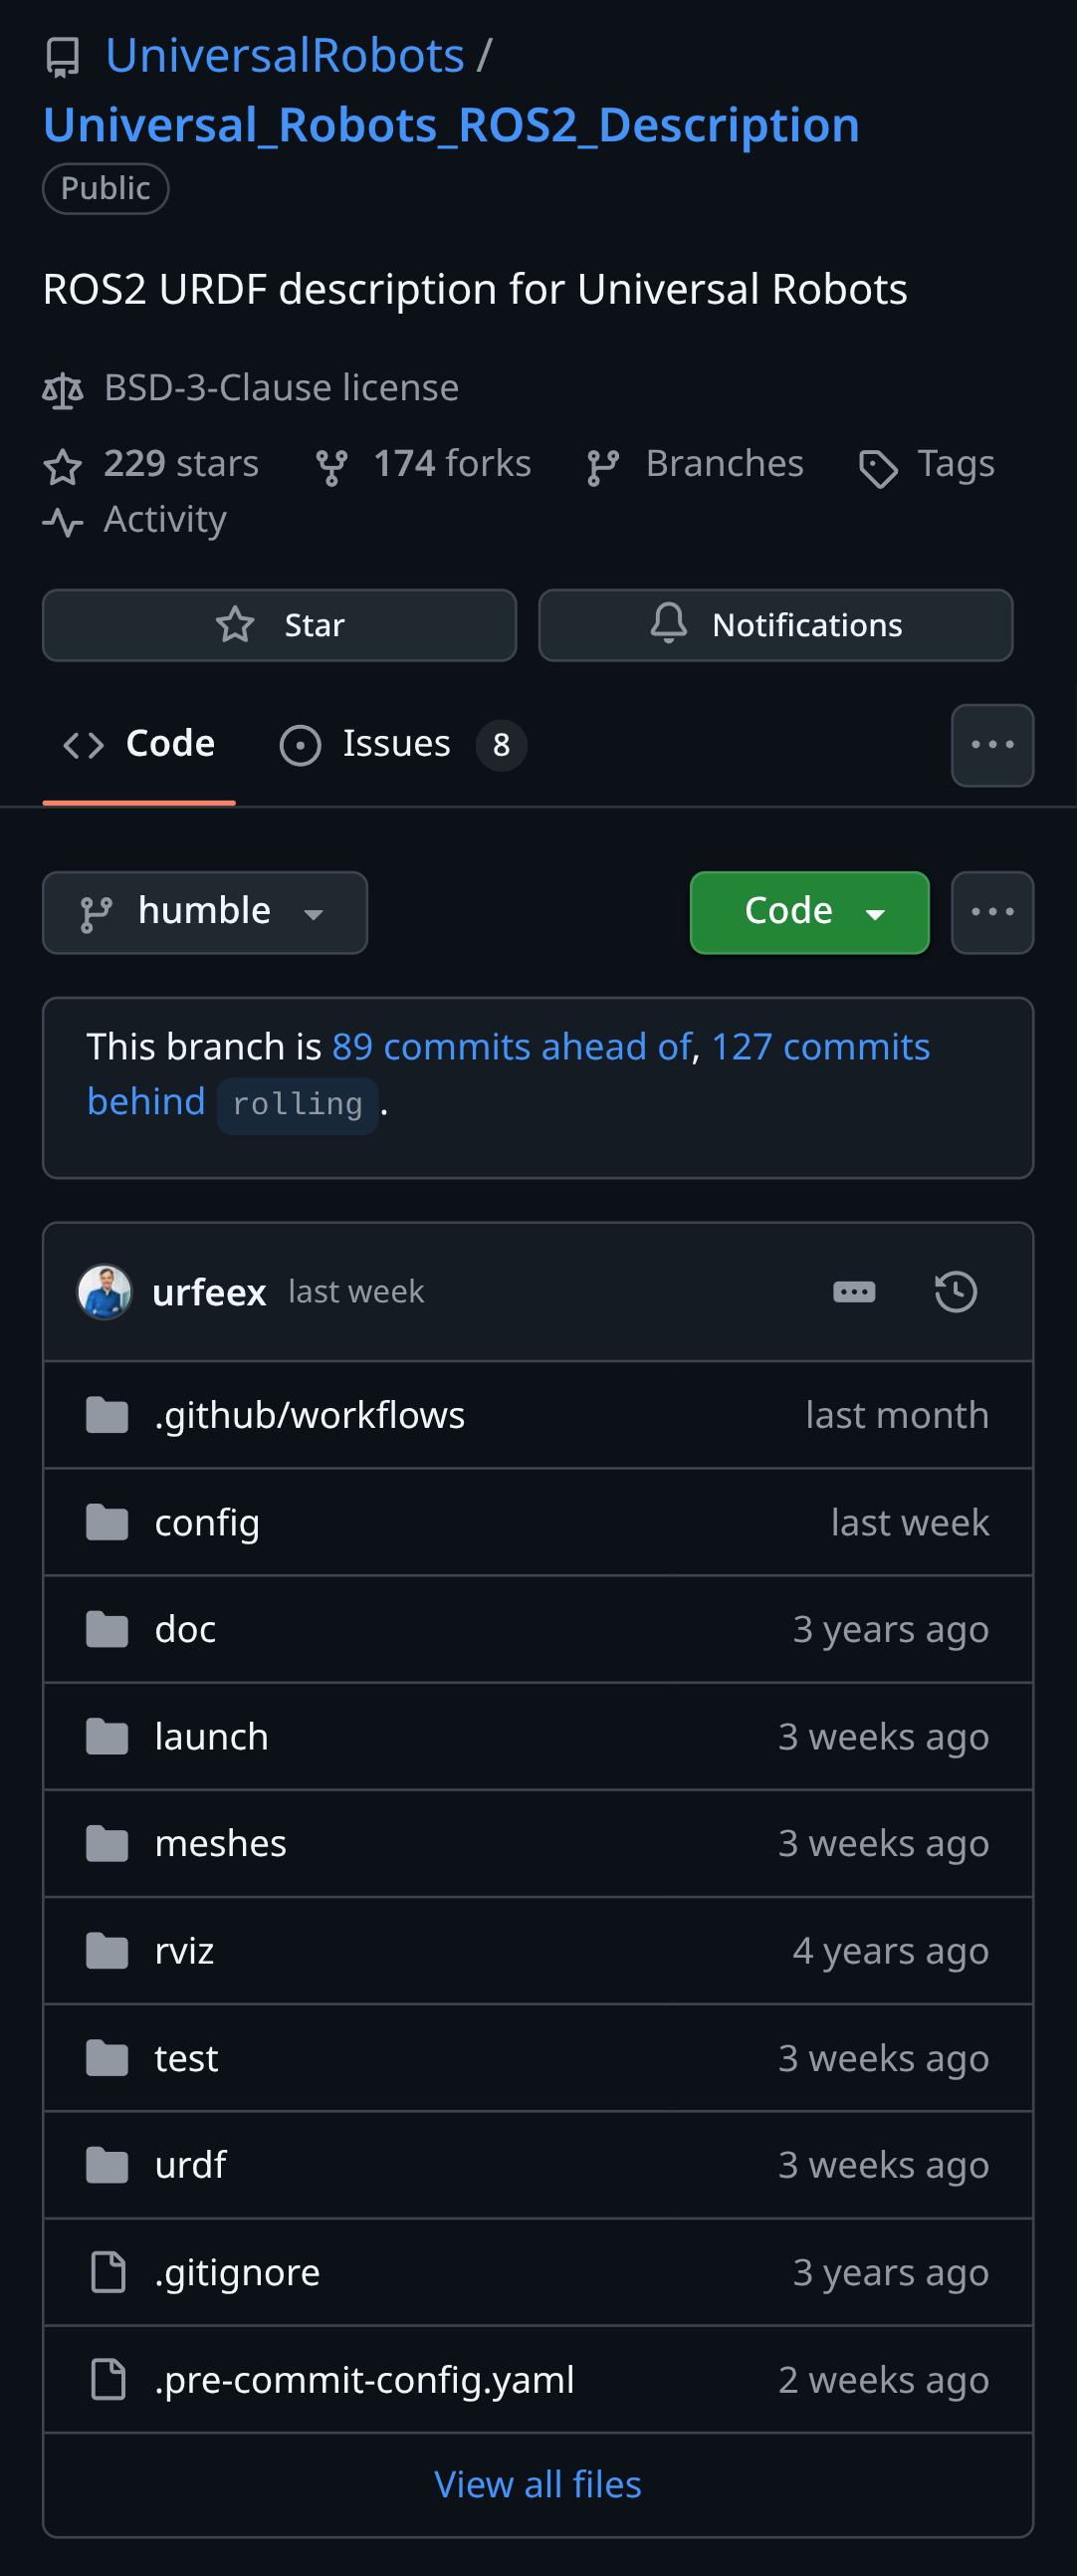
\includegraphics[width=.75\textwidth]{media/UR5DescriptionRepo.png}
            \end{center}
        \end{column}
    \end{columns}
\end{frame}
\begin{frame}{Gripper Description}
    \begin{columns}
        \begin{column}{.75\linewidth}
            The Robotiq 2f85 Gripper Description comes from the \href{https://github.com/PickNikRobotics/ros2_robotiq_gripper/tree/humble}{``Humble'' branch of the PickNikRobotics' GitHub repository}.

            Several modifications were made to the original URDF to allow for the Gazebo Simulation, which was initially not supported.
        \end{column}
        \begin{column}{.25\linewidth}
            \begin{center}
                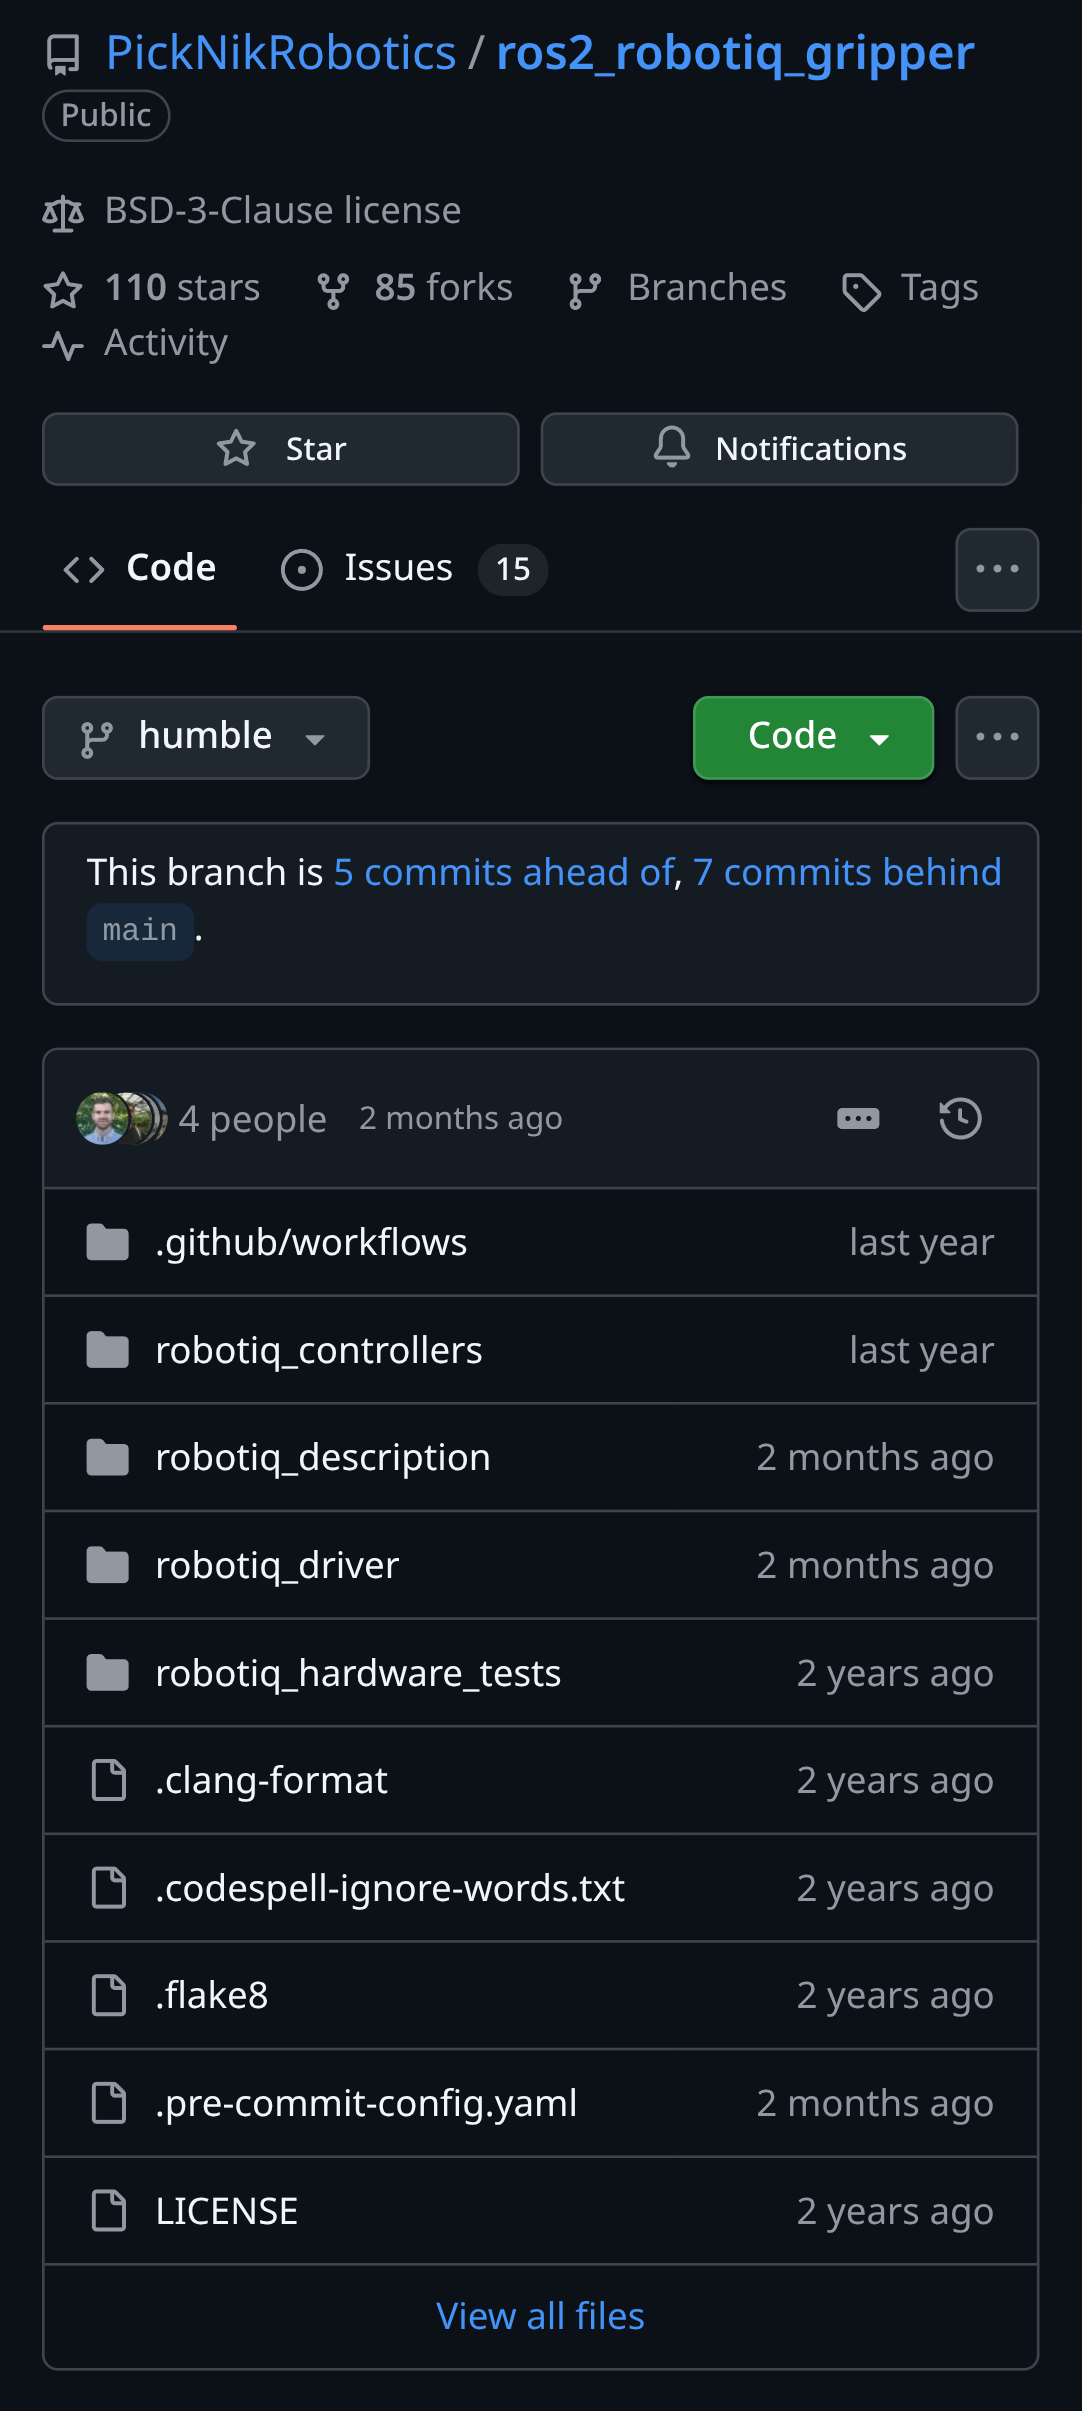
\includegraphics[width=.75\textwidth]{media/RobotiqGripperDescriptionRepo.png}
            \end{center}
        \end{column}
    \end{columns}
\end{frame}
\begin{frame}{Robot Controllers}
    The controllers used were the ones from the description repositories, grouped in a single file for ease of use.

    This means that the MoveIt2 dummy controllers were to be replaced in the final MoveIt Configuration Package.

    Especially the Joint Trajectory Controller and the Gripper Action Controller were useful for the project purposes.
\end{frame}
\begin{frame}{Depth Camera Description}
    The Depth camera is entirely simulated:
    \begin{itemize}
        \item $1024px \times 768px$ Resolution
        \item $2.24\mu m \times 2.24\mu m$ pixels
        \item Minimum perceived depth of $0.10 m$
        \item Maximum perceived depth of $2.25 m$
    \end{itemize}
    It is positioned $2m$ above and $50cm$ in front of the Base Link of the Robot, while pointing down.
\end{frame}
\begin{frame}{Gazebo World}
    \begin{columns}
        \begin{column}{.5\linewidth}
            The world consists in three objects:
            \begin{itemize}
                \item Robot Base
                \item Target Base
                \item Target
            \end{itemize}
        \end{column}
        \begin{column}{.5\linewidth}
            \begin{center}
                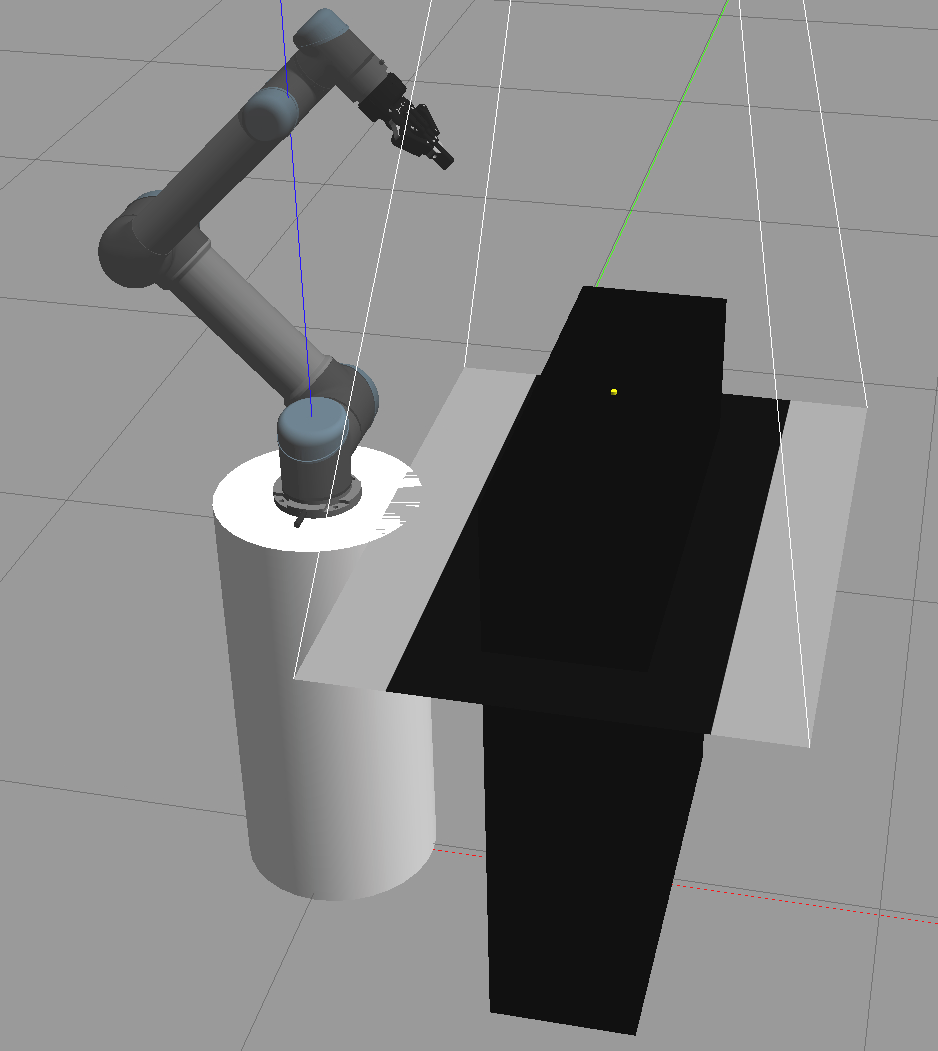
\includegraphics[width=.75\textwidth]{media/GazeboWorld.png}
            \end{center}
        \end{column}
    \end{columns}
\end{frame}
\begin{frame}{MoveIt Setup - Move Groups and Controllers}
    Two move groups:
    \begin{enumerate}
        \item ``\texttt{ur\textunderscore manipulator}'' $\rightarrow$ The UR5 Manipulator
        \item ``\texttt{ur\textunderscore gripper}'' $\rightarrow$ The Robotiq 2f85 Gripper
    \end{enumerate}
    Two ROS2 controllers:
    \begin{enumerate}
        \item ``\texttt{joint\textunderscore trajectory\textunderscore controller}'' $\rightarrow$ \texttt{JointTrajectoryController}
        \item ``\texttt{gripper\textunderscore position\textunderscore controller}'' $\rightarrow$ \texttt{GripperActionController}
    \end{enumerate}
    Two MoveIt2 controllers:
    \begin{enumerate}
        \item ``\texttt{joint\textunderscore trajectory\textunderscore controller}'' $\rightarrow$ \texttt{FollowJointTrajectory}
        \item ``\texttt{gripper\textunderscore position\textunderscore controller}'' $\rightarrow$ \texttt{GripperCommand}
    \end{enumerate}
\end{frame}
\begin{frame}{MoveIt Setup - Motion Planners}
    Adapted using the correct move groups from the MoveIt2 tutorials repository:
    \begin{itemize}
        \item ``\texttt{chomp\textunderscore planning.yaml}''
        \item ``\texttt{lerp\textunderscore planning.yaml}''
        \item ``\texttt{ompl\textunderscore planning.yaml}''
        \item ``\texttt{pilz\textunderscore industrial\textunderscore motion\textunderscore planner\textunderscore planning.yaml}''
        \item ``\texttt{trajopt\textunderscore planning.yaml}''
    \end{itemize}
\end{frame}
\begin{frame}{Running the Inverse Kinematics}
    \begin{columns}
        \begin{column}{.5\linewidth}
            The Inverse Kinematics is ran using the MoveIt2 APIs in a C++ ROS2 node.
        \end{column}
        \begin{column}{.5\linewidth}
            \inputminted[
                fontsize=\tiny,
                breaklines,
                firstline=174,
                lastline=180
            ]{c++}{../ros-humble-sim_workspace/ws_ur/src/ur_gripper_sim/src/run_ik.cpp}   
        \end{column}
    \end{columns}
\end{frame}
\begin{frame}{Running the Inverse Kinematics}
    \begin{columns}
        \begin{column}{.25\linewidth}
            The world objects geometries are added to the planning scene for the Motion Planner to avoid them.
        \end{column}
        \begin{column}{.75\linewidth}
            \inputminted[
                fontsize=\tiny,
                breaklines,
                firstline=190,
                lastline=213
            ]{c++}{../ros-humble-sim_workspace/ws_ur/src/ur_gripper_sim/src/run_ik.cpp}   
        \end{column}
    \end{columns}
\end{frame}
\begin{frame}{Running the Inverse Kinematics}
    \begin{columns}
        \begin{column}{.35\linewidth}
            The object contours coordinates are loaded into a ``\texttt{pts}'' vector, and the waypoints are computed by combining such coordinates and a predefined target orientation.
        \end{column}
        \begin{column}{.65\linewidth}
            \inputminted[
                fontsize=\tiny,
                breaklines,
                firstline=233,
                lastline=236
            ]{c++}{../ros-humble-sim_workspace/ws_ur/src/ur_gripper_sim/src/run_ik.cpp}
            \inputminted[
                fontsize=\tiny,
                breaklines,
                firstline=238,
                lastline=239
            ]{c++}{../ros-humble-sim_workspace/ws_ur/src/ur_gripper_sim/src/run_ik.cpp}
            \inputminted[
                fontsize=\tiny,
                breaklines,
                firstline=242,
                lastline=252
            ]{c++}{../ros-humble-sim_workspace/ws_ur/src/ur_gripper_sim/src/run_ik.cpp}
        \end{column}
    \end{columns}
\end{frame}
\begin{frame}{Running the Inverse Kinematics}
    \begin{columns}
        \begin{column}{.35\linewidth}
            Finally, a cartesian path is computed and the trajectory with its timing law is executed.
        \end{column}
        \begin{column}{.65\linewidth}
            \inputminted[
                fontsize=\tiny,
                breaklines,
                firstline=254,
                lastline=265
            ]{c++}{../ros-humble-sim_workspace/ws_ur/src/ur_gripper_sim/src/run_ik.cpp}
            \inputminted[
                fontsize=\tiny,
                breaklines,
                firstline=267,
                lastline=269
            ]{c++}{../ros-humble-sim_workspace/ws_ur/src/ur_gripper_sim/src/run_ik.cpp}
        \end{column}
    \end{columns}
\end{frame}
\section{Path Predictor Setup}
\label{Sec:PathPredictor_Setup}
\begin{frame}{ROS Package}
    Used to gather the image and depth data from the Depth Camera Node, which publishes:
    \begin{itemize}
        \item Color image on ``\texttt{/depth\textunderscore camera/image\textunderscore raw}''
        \item Greyscale depth image on ``\texttt{/depth\textunderscore camera/depth/image\textunderscore raw}''
        \item PointCloud on ``\texttt{/depth\textunderscore camera/points}''
    \end{itemize}
    And store such data in files in the Common Workspace.
\end{frame}
\begin{frame}{Python Application - Bootstrapper}
    \begin{columns}
        \begin{column}{.25\linewidth}
            The bootstrapper launches three scripts:
            \begin{enumerate}
                \item Contour detector
                \item Pixel to World coordinates Converter
                \item Duplicate Remover
            \end{enumerate}
        \end{column}
        \begin{column}{.75\linewidth}
            \inputminted[
                fontsize=\tiny,
                breaklines,
                firstline=15,
                lastline=35
            ]{python}{../path-predictor_workspace/predict.py}
        \end{column}
    \end{columns}
\end{frame}
\begin{frame}{Python Application - Contour Detector}
    \begin{columns}
        \begin{column}{.4\linewidth}
            The detector uses \texttt{OpenCV} to find object contours by thresholding the image's pixels RGB values and finding closed paths.

            After some candidates are found, the program shows a window with the image and the different objects with their contours highlighted. The user is finally asked which one is the object of interest before dumping its contour's pixels into the output file.
        \end{column}
        \begin{column}{.6\linewidth}
            \begin{figure}
                \begin{center}
                    \begin{subfigure}{\textwidth}
                        \centering
                        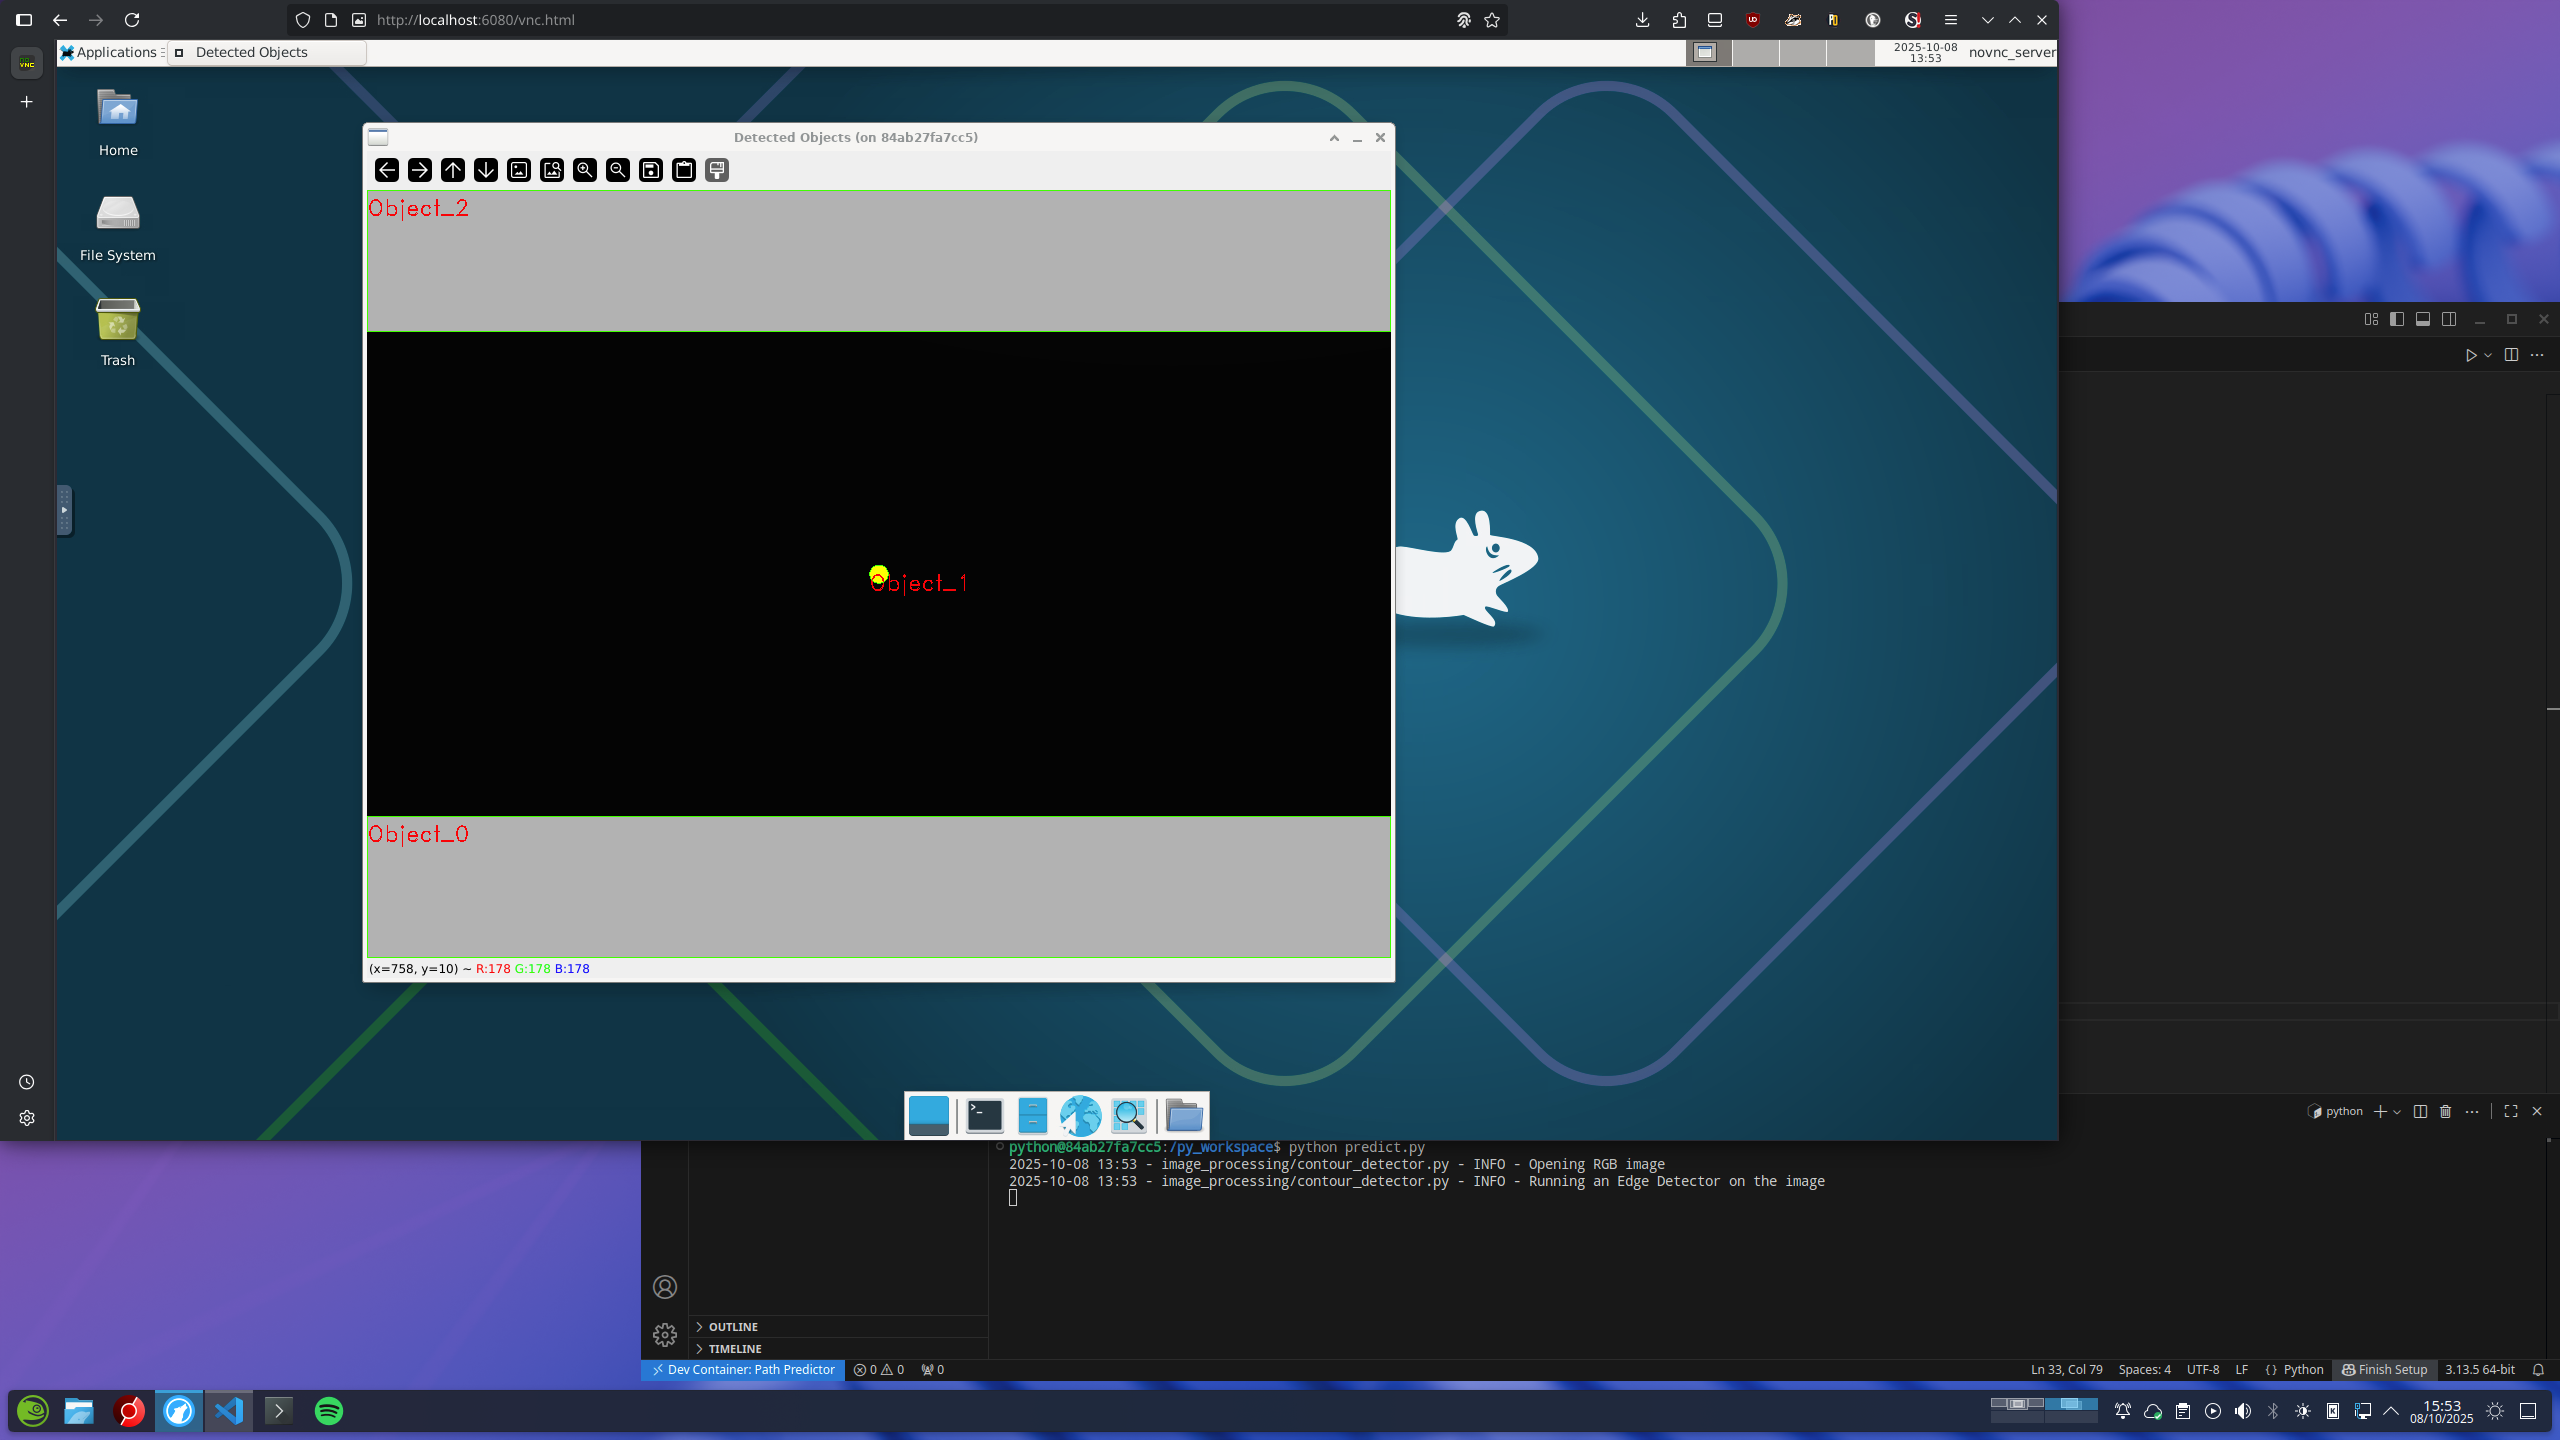
\includegraphics[width=\textwidth]{media/ContourDetector_Detection.png}
                    \end{subfigure}
                    \begin{subfigure}{\textwidth}
                        \centering
                        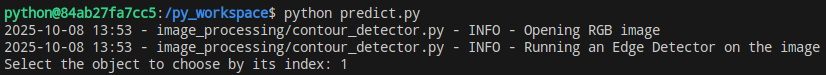
\includegraphics[width=\textwidth]{media/ContourDetector_Prompt.png}
                    \end{subfigure}
                \end{center}
            \end{figure}
        \end{column}
    \end{columns}
\end{frame}
\begin{frame}{Python Application - Pixel to World coordinates Converter}
    \begin{columns}
        \begin{column}{.35\linewidth}
            Given the simulated camera intrinsic and extrinsic parameters it computes the correspondance between the pixel coordinates and the simulated world 3D coordinates, using both the contour's pixels coordinates and the depth data coming from the PointCloud published by the depth camera itself.
        \end{column}
        \begin{column}{.65\linewidth}
            \inputminted[
                fontsize=\tiny,
                breaklines,
                firstline=234,
                lastline=237
            ]{python}{../path-predictor_workspace/image_processing/pixel_to_world.py}
            \inputminted[
                fontsize=\tiny,
                breaklines,
                firstline=239,
                lastline=242
            ]{python}{../path-predictor_workspace/image_processing/pixel_to_world.py}
            \inputminted[
                fontsize=\tiny,
                breaklines,
                firstline=245,
                lastline=258
            ]{python}{../path-predictor_workspace/image_processing/pixel_to_world.py}
        \end{column}
    \end{columns}
\end{frame}
\begin{frame}{Python Application - Duplicate Remover}
    \begin{columns}
        \begin{column}{.50\linewidth}
            Since there's the possibility that different pixels map to the same coordinates after the rounding to millimetric precision, the consecutive duplicates are dropped from the final object contour coordinates file.
        \end{column}
        \begin{column}{.50\linewidth}
            \inputminted[
                fontsize=\tiny,
                breaklines,
                firstline=55,
                lastline=65
            ]{python}{../path-predictor_workspace/image_processing/duplicate_remover.py}
        \end{column}
    \end{columns}
\end{frame}
\section{Usage}
\label{Sec:Usage}
\begin{frame}[fragile]{Usage Pipeline}
    \begin{enumerate}
        \item \textbf{Spawn the Robot with the depth camera and take pictures} \par
        \begin{minted}[
            fontsize=\footnotesize,
            breaklines
        ]{bash}
ros@ros_devcontainer:~$ ros2 launch ur_gripper_sim get_data_w{i}.launch.py
        \end{minted}
        \item \textbf{Predict the contours of the object} \par
        \begin{minted}[
            fontsize=\footnotesize,
            breaklines
        ]{bash}
py@python_devcontainer:~$ python ./predict.py
        \end{minted}
        \item \textbf{Spawn the Robot with the MoveIt2 Controllers and run the Inverse Kinematics} \par
        \begin{minted}[
            fontsize=\footnotesize,
            breaklines
        ]{bash}
# Terminal Window 1
ros@ros_devcontainer:~$ ros2 launch ur_gripper_sim sim_w{i}.launch.py
# Terminal Window 2
## Run the node once the simulation environment is ready
ros@ros_devcontainer:~$ ros2 run ur_gripper_sim run_ik
        \end{minted}
    \end{enumerate}
\end{frame}
\begin{frame}[standout]
    \thispagestyle{empty}
    Demo
\end{frame}
\begin{frame}[standout]
    \thispagestyle{empty}
    Thank you.
\end{frame}
\begin{frame}[allowframebreaks]{Bibliography}
    \nocite{*}
    \bibliography{references}
    \bibliographystyle{unsrt}
\end{frame}

\end{document}